\subsection{Fabricating Supporting Structures}
The sections below provide drawings with labelled dimensions and tables with the corresponding measurements. Measure the procured components and apply the dimensions to the drawings to identify suitable supporting structures for your components.


\subsubsection{3D Printing}

If you have access to a 3D printer, then check (XX APENDIX x) to see the measurements used to create the STL files for the components. If your component parts have the same measurements, then use the supplied files. If component measurements vary then use the drawings to design your own, at the time of writing Autodesk provide a free version of Autodesk that can be used to design the parts and export to STL files for printing. Aim to use a stiff setting filament to optimise the transmission of load for loadcell measurement.
\subsubsection{Workshop Manufacturing}

Use the drawings and relative measurements in each section to form the design for each part. Aim to use lightweight and stiff materials, this will ensure that the load transmission for measurement via loadcells is optimised.

\clearpage
\subsubsection{Uroflowmetry Base Plates}

The drawings below outline base plates fit for purpose, two are required. The large flat bottom provides a large stable base in contact with the floor as well as a large pad to place the fluid container on. 
The design centres the loadcell in the middle of the plate so that the weight of the container and fluid are over the centre of the plate. This reduces the likelihood of the container falling over if knocked.

\begin{figure}[h]
    \centering
    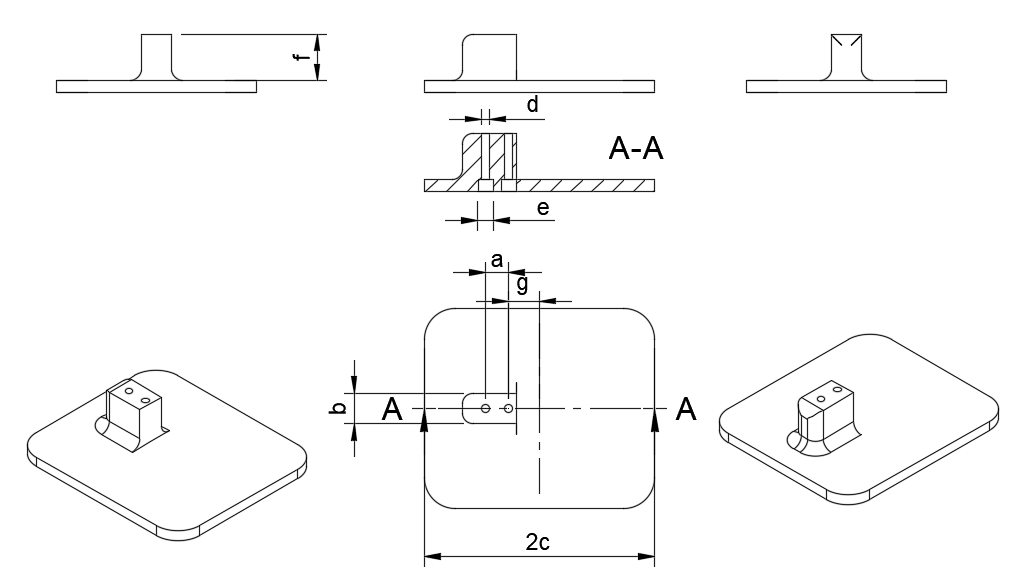
\includegraphics[width=0.7\textwidth]{Figures/SupportDrawings/uf_base_plate_drawing.png}
    \caption{Uroflowmetry Base Plate Drawings}
    \label{fig:ufbaseplatedrawing}
  \end{figure}

  \begin{enumerate}
    \item[a)] The distance between the centre points of the two tapped holes at each end of the loadcell
    \item[b)] The width of the loadcell + \textgreater\ 2mm
    \item[c)] Length of the loadcell
    \item[d)] The bolt diameter used by the loadcell + \textgreater\ 1mm
    \item[e)] The diameter of the head of the bolt + \textgreater\ 2mm 
    \item[f)] The height of the loadcell
    \item[g)] Distance between the centre of the loadcell and the centre point of the loadcell hole nearer to the loadcell mid-point
  \end{enumerate}
\clearpage
\subsubsection{Pressure Configuration Clamp Design}

The drawings below outline the pressure configuration clamp, two are required. Two of these can be fixed together on a stand to provide a clamp for the pressure sensor syringes. 
The four bolt and nut holes allow the two parts to be clamped together around the upright support. The internal nut holes and through bolt holes allow a single bolt ant nut to act as grub screws to fix the two syringes in place and fix the clamp to the upright support. The single nut and bolt hole  at the end of the part clamps the two parts together so that the syringe grub screws do not splay the parts. 


\begin{figure}[h]
    \centering
    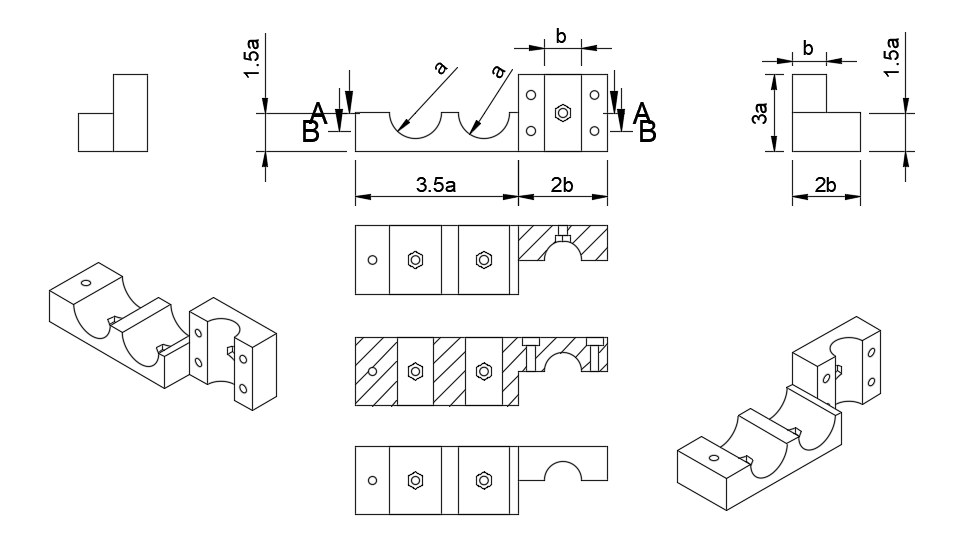
\includegraphics[width=0.7\textwidth]{Figures/SupportDrawings/pressure_conf_clamp_drawing.png}
    \caption{Pressure Syringe Clamp Drawings}
    \label{fig:pressuresyringeclampdrawing}
  \end{figure}


\begin{enumerate}
  \item[a)] The diameter of the pressure syringe + \textgreater\ 4mm
  \item[b)] The diameter of the upright stand/trolley + \textgreater\ 4mm
  \item[Nb)] Select bolts that are greater than the larger of 3a and 3b
  \item[Nb)] Create holes to accommodate the chosen bolts
  \item[Nb)] Create hexagonal holes to accommodate the corresponding nuts, a tight fit makes it easier to move the bolts without the nuts dropping out
\end{enumerate}

\clearpage
\subsubsection{Infusion Pump Clamp Design}

The drawings below outline the infusion pump clamp, two are required. Two of these can be fixed together on a stand to provide a clamp for the infusion pump to be fixed to. 
The four bolt and nut holes allow the two parts to be clamped together around the upright support. The internal nut hole and through bolt hole allow a single bolt ant nut to act as grub screw to fix the clamp to the upright support. The two through holes allow bolts to pass through the part to fix the pump to the clamp.


\begin{figure}[h]
    \centering
    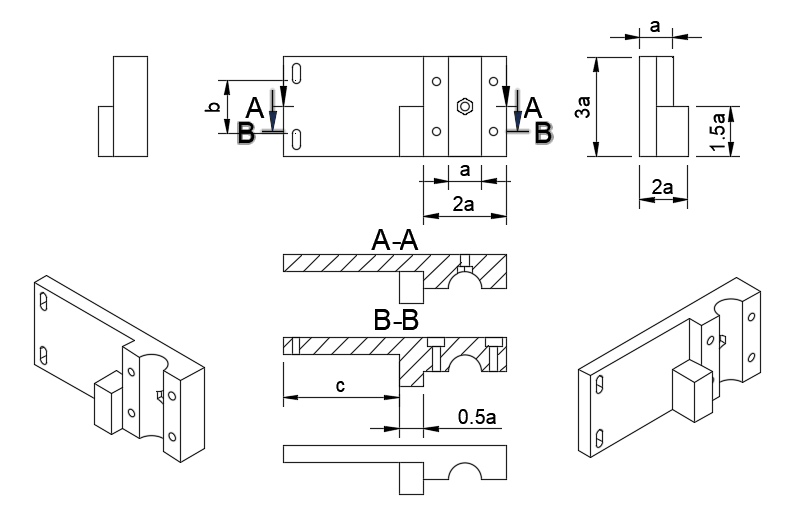
\includegraphics[width=0.7\textwidth]{Figures/SupportDrawings/inf_pump_clamp_drawing.png}
    \caption{Infusion Pump Clamp Drawings}
    \label{fig:infpumpclampdrawing}
  \end{figure}

\begin{enumerate}
  \item[a)]	The diameter of the upright stand/trolley + \textgreater\ 4mm
  \item[b)]	The distance between the pump fixation screw holes - 5mm
  \item[c)]	The length of the pump + \textgreater\ 10mm
\end{enumerate}


\clearpage
\subsubsection{Volume Infused Loadcell Clamp Design}

The drawings below outline the fluid infusion loadcell clamp, two are required. Two of these can be fixed together on a stand to provide a clamp for the fluid infusion loadcell.
The four bolt and nut holes allow the two parts to be clamped together around the upright support. The internal nut hole and through bolt hole allow a single bolt ant nut to act as grub screw to fix the clamp to the upright support. The two through holes allow bolts to pass through the part to fix the loadcell to the clamp.


\begin{figure}[h]
    \centering
    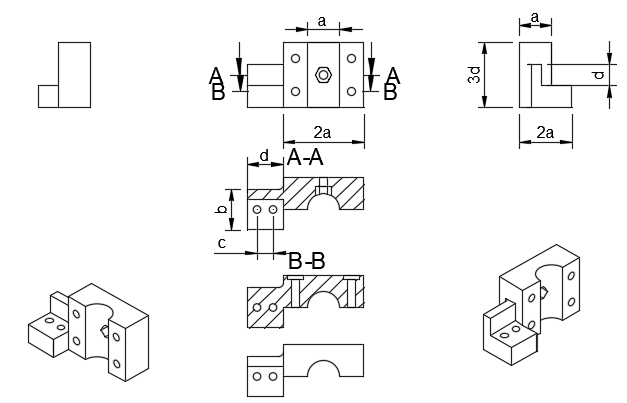
\includegraphics[width=0.7\textwidth]{Figures/SupportDrawings/vol_inf_loadcell_clamp_drawing.png}
    \caption{Volume Infused Loadcell Clamp Drawings}
    \label{fig:viloadcellclampdrawing}
  \end{figure}

\begin{enumerate}
  \item[a)] The diameter of the upright stand/trolley + \textgreater\ 4mm
  \item[b)] Twice the width of the loadcell + 4mm
  \item[c)] The distance between the centre points of the two tapped holes at each end of the loadcell
  \item[d)] Height of the loadcell
  \item[Nb.] Create holes to accommodate the chosen bolts
  \item[Nb.] Create hexagonal holes to accommodate the corresponding nuts, a tight fit makes it easier to move the bolts without the nuts dropping out
\end{enumerate}
\clearpage
\subsubsection{Volume Infused Fluid Mount Clamp Design}

The drawings below outline the fluid infusion mount, one part is required. The part is fixed to the end of the fluid infusion load cell and allows the infusion bag to be supported and weighed.
The two through holes allow bolts to pass through the part to fix the loadcell to the clamp. The upright cylinder/hook acts as the point to fix the infusion fluid bag, it should be made sufficiently strong to hold a minimum of 1.25 kg.


\begin{figure}[h]
    \centering
    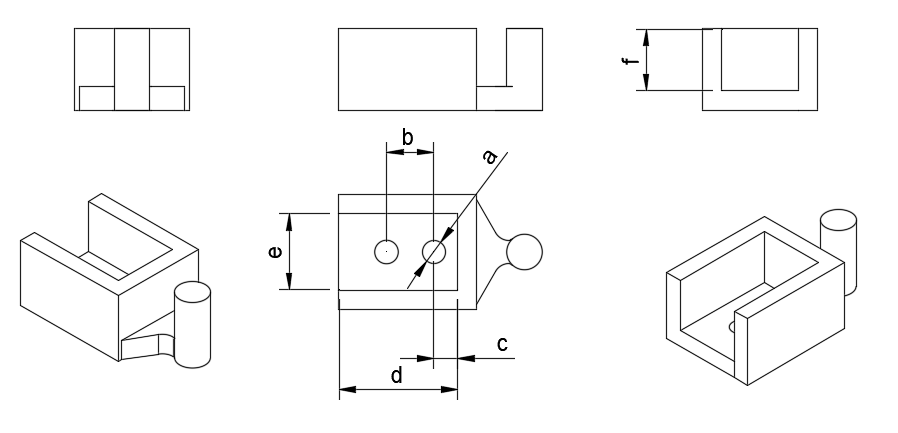
\includegraphics[width=0.7\textwidth]{Figures/SupportDrawings/vi_fluid_bag_mount_drawing.png}
    \caption{Volume Infused Fluid Mount Clamp Drawings}
    \label{fig:vimountclampdrawing}
  \end{figure}


  \begin{enumerate}
    \item[a)] The diameter of the upright stand/trolley + \textgreater\ 4mm
    \item[a)]	The bolt diameter used by the loadcell + \textgreater\ 1mm
    \item[b)]	The distance between the centre points of the two tapped holes at each end of the loadcell
    \item[c)]	The distance between the centre points loadcells outermost hole and the end of the loadcell + 1mm
    \item[d)]	Distance from the end of the loadcell to the innermost holes edge + \textgreater\ 5mm
    \item[e)]	The width of the loadcell + 4mm
    \item[f)]	Height of the loadcell

  \end{enumerate}


\clearpage